\documentclass{article}
\usepackage[utf8x]{inputenc}
\usepackage{ucs}
\usepackage{amsmath} 
\usepackage{amsfonts}
\usepackage{marvosym}
\usepackage{wasysym}
\usepackage{upgreek}
\usepackage[english,russian]{babel}
\usepackage{graphicx}
\usepackage{float}
\usepackage{textcomp}
\usepackage{hyperref}
\usepackage{geometry}
  \geometry{left=2cm}
  \geometry{right=1.5cm}
  \geometry{top=1cm}
  \geometry{bottom=2cm}
\usepackage{tikz}
\usepackage{ccaption}
\usepackage{multicol}
\usepackage[shortlabels]{enumitem}

\hypersetup{
   colorlinks=true,
   citecolor=blue,
   linkcolor=black,
   urlcolor=blue
}

\usepackage{listings}
%\setlength{\columnsep}{1.5cm}
%\setlength{\columnseprule}{0.2pt}

\usepackage[absolute]{textpos}


\usepackage{colortbl,graphicx,tikz}
\definecolor{X}{rgb}{.5,.5,.5}

\renewcommand{\thesubsection}{\arabic{subsection}}

\begin{document}
\pagenumbering{gobble}
\lstset{
  language=C,                % choose the language of the code
  basicstyle=\linespread{1.1}\ttfamily,
  columns=fixed,
  fontadjust=true,
  basewidth=0.5em,
  keywordstyle=\color{blue}\bfseries,
  commentstyle=\color{gray},
  stringstyle=\ttfamily\color{orange!50!black},
  showstringspaces=false,
  numbersep=5pt,
  numberstyle=\tiny\color{black},
  numberfirstline=true,
  stepnumber=1,                   % the step between two line-numbers.        
  numbersep=10pt,                  % how far the line-numbers are from the code
  backgroundcolor=\color{white},  % choose the background color. You must add \usepackage{color}
  showstringspaces=false,         % underline spaces within strings
  captionpos=b,                   % sets the caption-position to bottom
  breaklines=true,                % sets automatic line breaking
  breakatwhitespace=true,         % sets if automatic breaks should only happen at whitespace
  xleftmargin=.2in,
  extendedchars=\true,
  keepspaces = true,
}
\lstset{literate=%
   *{0}{{{\color{red!20!violet}0}}}1
    {1}{{{\color{red!20!violet}1}}}1
    {2}{{{\color{red!20!violet}2}}}1
    {3}{{{\color{red!20!violet}3}}}1
    {4}{{{\color{red!20!violet}4}}}1
    {5}{{{\color{red!20!violet}5}}}1
    {6}{{{\color{red!20!violet}6}}}1
    {7}{{{\color{red!20!violet}7}}}1
    {8}{{{\color{red!20!violet}8}}}1
    {9}{{{\color{red!20!violet}9}}}1
}

\renewcommand{\thesubsection}{\arabic{subsection}}
\makeatletter
\def\@seccntformat#1{\@ifundefined{#1@cntformat}%
   {\csname the#1\endcsname\quad}%    default
   {\csname #1@cntformat\endcsname}}% enable individual control
\newcommand\section@cntformat{}     % section level 
\newcommand\subsection@cntformat{Задача \thesubsection.\space} % subsection level
\newcommand\subsubsection@cntformat{\thesubsubsection.\space} % subsubsection level
\makeatother


\makeatletter
\newcount\my@repeat@count
\newcommand{\myrepeat}[2]{%
  \begingroup
  \my@repeat@count=\z@
  \@whilenum\my@repeat@count<#1\do{#2\advance\my@repeat@count\@ne}%
  \endgroup
}
\makeatother

\title{Семинар \#3: Строки. Домашнее задание.\vspace{-5ex}}\date{}\maketitle

\subsection{Тип символа}
Напишите программу, которая будет считывать символ и печатать:
\begin{itemize}
\item \texttt{Letter}, если этот символ – буква (\texttt{[A, Z]} и \texttt{[a, z]})
\item \texttt{Digit}, если этот символ – цифра
\item \texttt{Other}, если это какой-то другой символ
\end{itemize}

Решите эту задачу в трёх вариантах:
\begin{enumerate}[(a)]
\item Без использования строковых литералов и библиотеки \texttt{ctype.h}
\item Используя строковые литералы, но без использования библиотеки \texttt{ctype.h}
\item Используя библиотеку \texttt{ctype.h}
\end{enumerate}



\subsection{Чередование}
Считать 2 слова и печатать их чередуя по одному символу. То есть сначала напечатать первый символ первой строки, потом первый символ второй строки, потом второй символ первой строки, второй символ второй и т. д. Если какая-то из строк закончится, то нужно допечатать оставшуюся строку.
\begin{center}
\begin{tabular}{ l | l }
 вход & выход \\ \hline
 \texttt{cat dog} & \texttt{cdaotg}  \\ 
 \texttt{cat elephant} & \texttt{cealtephant} \\
 \texttt{elephant dog} & \texttt{edloegphant} \\
 \texttt{aaaa bbbb} & \texttt{abababab} \\
 \texttt{aaaa b} & \texttt{abaaa}\\ 
 \texttt{a b} & \texttt{ab}\\ 
\end{tabular}
\end{center}



\subsection{Палиндром}
Написать функцию \texttt{is\_palindrom}, которая будет принимать строку и проверять является ли эта строка палидромом.

\begin{multicols}{2}
\begin{center}
\begin{tabular}{ l | l }
 вход & выход \\ \hline
 \texttt{abba} & \texttt{Yes} \\
 \texttt{aba} & \texttt{Yes} \\
 \texttt{a} & \texttt{Yes} \\
 \texttt{aa} & \texttt{Yes} \\
 \texttt{ab} & \texttt{No} 
\end{tabular}
\end{center}


\begin{center}
\begin{tabular}{ l | l }
 вход & выход \\ \hline
 \texttt{abcdedcba} & \texttt{Yes} \\
 \texttt{abcdedcb} & \texttt{No} \\
 \texttt{abcdedcbab} & \texttt{No} \\
 \texttt{abcdedcbb} & \texttt{No} \\
 \texttt{abcxedcba} & \texttt{No}
\end{tabular}
\end{center}
\end{multicols}

\subsection{Шифр Цезаря}
Шифр Цезаря — это вид шифра подстановки, в котором каждый символ заменяется символом, находящимся на некотором постоянном числе позиций левее или правее него в алфавите. 
\begin{center}
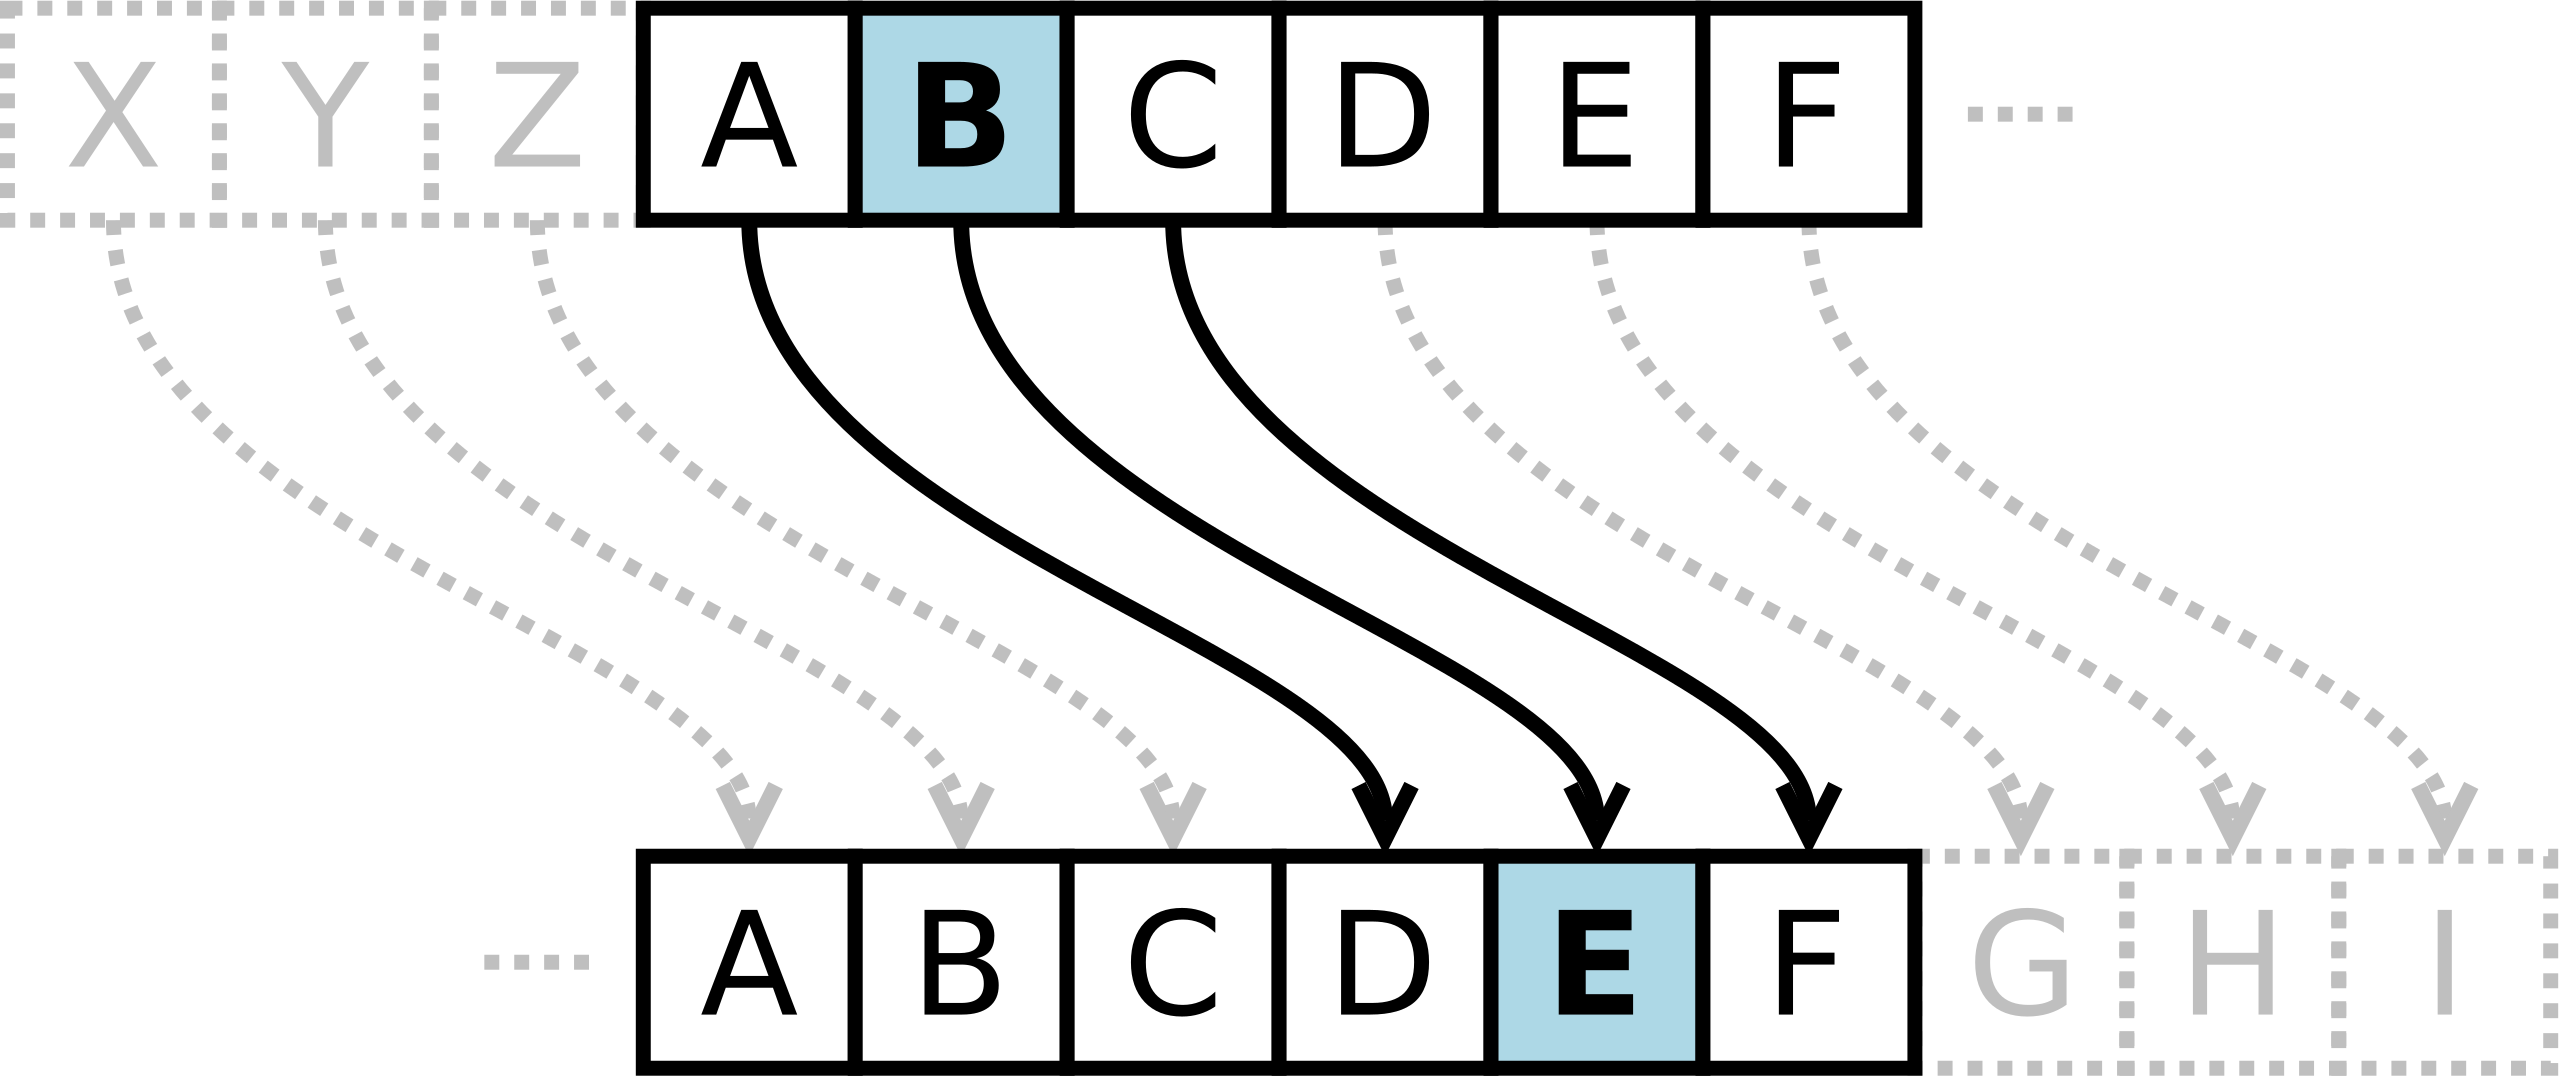
\includegraphics[width=0.4\textwidth]{../images/caesar.png}
\end{center}
Напишите функцию \texttt{void encrypt(char* str, int k)}, которая будет зашифровывать фразу шифром Цезаря.
\begin{center}
\begin{tabular}{ c | c }
 вход & выход \\ \hline
 \texttt{1 ABCZ} & \texttt{BCDA}\\
 \texttt{15 ZzZzZ} & \texttt{OoOoO} \\
 \texttt{7 The Fox Jumps Over The Dog} & \texttt{Aol Mve Qbtwz Vcly Aol Kvn} \\
 \texttt{13  Green Terra} & \texttt{Terra Green}
\end{tabular}
\end{center}


\subsection{Укоротить строку}
Напишите функцию \texttt{void trim\_after\_first\_space(char str[])}, которая будет принимать на строку и укорачивать её до первого пробела. Протестируйте функцию с помощью следующего кода:
\begin{lstlisting}
#include <stdio.h>
// Тут вам нужно написать функцию trim_after_first_space
int main() 
{
    char a[] = "Cats and Dogs";
    printf("%s\n", a); // Должно напечатать Cats and Dogs
    trim_after_first_space(a);
    printf("%s\n", a); // Должно напечатать Cats
}
\end{lstlisting}


\subsection{Сокровище}
Вы находитесь на плоскости в начале координат (точке с координатами \texttt{(0, 0)}) и вам нужно найти закопанное сокровище. Путь до него задаётся последовательностью команд, состоящих из направления и расстояния, которое нужно пройти в этом направлении. Вам нужно найти координаты сокровища. Используйте функцию \texttt{strcmp}.
\begin{center} 
\begin{tabular}{ l | l }
 вход & выход \\ \hline
 \texttt{6} & \texttt{-30 20}\\
 \texttt{North 10} & \\
 \texttt{East 20} &\\
 \texttt{South 50} &\\
 \texttt{West 60} &\\
 \texttt{East 10} &\\
 \texttt{North 60} &\\
\end{tabular}
\end{center}


\subsection{Безопасный \texttt{strcpy}}
Известно, что функция \texttt{strcpy} небезопасна, так как может выйти за границы массива, в который она записывает.
Например, в следующем примере:
\begin{lstlisting}
char a[10] = "Mouse";
char b[50] = "LargeElephant";
strcpy(a, b); // UB, выйдет за пределы массива a
\end{lstlisting}
Ваша задача заключается в том, чтобы написать функцию \texttt{safe\_strcpy}, которая будет более безопасной, чем функция \texttt{strcpy} и не будет выходить за границы массива. Эта функция должна иметь 3 параметра:
\begin{itemize}
\item строка в которую мы будем записывать (тип \texttt{char[]})
\item размер массива в который мы будем записывать (тип \texttt{size\_t})
\item строка из которой мы будем считывать (тип \texttt{const char[]}).
\end{itemize}
В случае если строка из которой мы считываем не будет помещаться в массив, нужно скопировать только часть строки, которая может поместиться в него. И обязательно поставить нулевой символ в конце строки.
\begin{lstlisting}
char a[10] = "Mouse";
char b[50] = "LargeElephant";
safe_strcpy(a, 10, b); // OK, строка a будет равна "LargeElep\0"
\end{lstlisting}



\subsection{Повторитель}
Напишите программу \texttt{repeater}, которая будет принимать через аргументы командной строки некоторое слово и некоторое число. Эта программа должна печатать это слово столько раз, чему равно переданное число.\\
Например, если мы вызовем эту программу так:
\begin{verbatim}
./repeater Hello 5
\end{verbatim}
то программа должна напечатать:
\begin{verbatim}
Hello Hello Hello Hello Hello
\end{verbatim}


\subsection{Сортировка аргументов}
Напишите программу \texttt{sort}, которая будет принимать через аргументы командной строки произвольное число строк и сортировать эти строки лексикографически и печатать их.\\
Например, если мы вызовем эту программу так:
\begin{verbatim}
./sort cat elephant mouse axolotl lion
\end{verbatim}
то программа должна напечатать:
\begin{verbatim}
axolotl cat elephant lion mouse
\end{verbatim}


\subsection{Шифрование файла}
Напишите программу \texttt{encrypt}, которая будет принимать через аргументы командной строки названия входного и выходного файлов, а также число-ключ шифра Цезаря. Программа должна считывать входной файл, зашифровывать его шифром Цезаря и записывать результат в выходной файл.\\
Например, если мы вызовем эту программу так:
\begin{verbatim}
./encrypt three_little_pigs.txt result.txt 7
\end{verbatim}
то программа должна считывать файл \texttt{three\_little\_pigs.txt}, зашифровывать содержимое шифром Цезаря с ключом 7 и записывать результат в файл \texttt{result.txt}.







\newpage
\section*{Необязательные задачи (не входят в ДЗ, никак не учитываются)}
\setcounter{subsection}{0}

\subsection{Номер буквы}
Считайте символ буквы латинского алфавита и напечатайте его номер в алфавите. Если на вход подаётся не буква, то нужно напечатать \texttt{Not a letter}.
\begin{center}
\begin{tabular}{ l | l }
 вход & выход \\ \hline
 \texttt{P} & \texttt{16} \\
 \texttt{b} & \texttt{2} \\
 \texttt{B} & \texttt{2} \\
 \texttt{\#} & \texttt{Not a letter}\\ 
\end{tabular}
\end{center}

\subsection{Лесенка}
Считать слово и напечатать лесенку из этого числа. Например, для слова \texttt{Hello} нужно напечатать лесенку: 
\begin{center}
\begin{center}
\begin{tabular}{ c | l }
 вход & выход \\ \hline
 \texttt{Hello} & \texttt{H}  \\ 
 & \texttt{He} \\
 & \texttt{Hel} \\
 & \texttt{Hell} \\
 & \texttt{Hello}\\ 
\end{tabular}
\end{center}
\end{center}



\subsection{Восклицание}
На вход подаётся строка. Напечатать эту же строку, но ставя восклицательный знак после каждого слова.
\begin{center}
\begin{tabular}{ l | l }
 вход & выход \\ \hline
 \texttt{Better late than never} & \texttt{Better! late! than! never!} \\
 \texttt{cat \quad dog elephant} & \texttt{cat! \quad dog! elephant!}  \\ 
 \texttt{a} & \texttt{a!} \\
\end{tabular}
\end{center}


\subsection{Правильная скобочная последовательность}
На вход подаётся скобочная последовательность(строка, состоящая из символов \texttt{'('} и \texttt{')'}). Нужно выяснить является ли эта скобочная последовательность допустимой или нет.
\begin{multicols}{2}
\begin{center}
\begin{tabular}{ l | l }
 вход & выход \\ \hline
 \texttt{(()())} & \texttt{Yes} \\
 \texttt{(()(()()))} & \texttt{Yes} \\
 \texttt{(()))()())} & \texttt{No} \\
 \texttt{(((())))} & \texttt{Yes} \\
 \texttt{(((()))))} & \texttt{No} \\
 \texttt{(((()))} & \texttt{No} \\
\end{tabular}
\end{center}

\begin{center}
\begin{tabular}{ l | l }
 вход & выход \\ \hline
 \texttt{()} & \texttt{Yes} \\
 \texttt{)(} & \texttt{No} \\
 \texttt{))} & \texttt{No} \\
 \texttt{((} & \texttt{No} \\
 \texttt{()()} & \texttt{Yes} \\
 \texttt{(} & \texttt{No} \\
 \texttt{)} & \texttt{No} \\
\end{tabular}
\end{center}
\end{multicols}


\subsection{Удаление символа}
Напишите функцию \texttt{void delete\_chars(char str[], char c)}, которая будет удалять все символы, равные \texttt{c} из строки \texttt{str}. Постарайтесь сделать эту функцию как можно более эффективной.

\begin{center}
\begin{tabular}{ l | l }
 \texttt{str, c} & \texttt{str} после вызова \texttt{delete\_chars(str, c)} \\ \hline
 \texttt{cat a} & \texttt{ct} \\
 \texttt{elephant e} & \texttt{lphant} \\
 \texttt{aaaa a} & \texttt{} \\
 \texttt{a a} & \texttt{} \\
 \texttt{ababababa a} & \texttt{bbbb} \\
\end{tabular}
\end{center}


\subsection{Самое длинное слово}
Напишите функцию \texttt{int longest\_word(const char str[], char result[])}, которая будет искать самое длинное слово в строке \texttt{str} и записывать его в строке \texttt{result}. Строка должна возвращать длину этого слова. Под словом тут понимается последовательность непробельных символов, ограниченная с двух сторон пробельными символами или границами строки.
В случае если есть несколько слов с самой большой длиной в \texttt{result} нужно записать первое из них.

\begin{center}
\begin{tabular}{ l | l }
 \texttt{str} & \texttt{result} после вызова \texttt{longest\_word(str, result)} \\ \hline
 \texttt{cats and dogs} & \texttt{cats} \\
 \texttt{cat dog elephant mouse} & \texttt{elephant} \\
 \texttt{cat \quad dog \quad\quad elephant mouse} & \texttt{elephant} \\
\end{tabular}
\end{center}

\subsection{Переворот слов в файле}
Счмтайте файл \texttt{input.txt}  и переверните все слова из этого файла и запишите результат в файл \texttt{output.txt}.
\begin{center} 
\begin{tabular}{ l | l }
 файл \texttt{input.txt} & файл \texttt{output.txt} \\ \hline
 \texttt{Cat and Dog} & \texttt{taC dna goD}\\
\end{tabular}
\end{center}
Протестируйте программу на файле \texttt{invisible\_man.txt}.






\subsection{*Замена}
Напишите программу \texttt{replacer}, которая будет принимать через аргументы командной строки названия входного и выходного файлов, а также две строки. Программа должна считывать входной файл, заменять все вхождения первой строки на вторую строку и записывать результат в выходной файл.\\
Например, если мы вызовем эту программу так:
\begin{verbatim}
./replacer three_little_pigs.txt result.txt pig elephant
\end{verbatim}
то программа должна считывать файл \texttt{three\_little\_pigs.txt}, заменять все подстроки \texttt{"pig"} на \texttt{"elephant"} и записывать результат в файл \texttt{result.txt}. Постарайтесь написать эффективный алгоритм замены. Рассмотите случаи когда подстрока заменяется на более длинную строку и когда подстрока заменяется на более короткую строку.

\end{document}